%\setcounter{chapter}{4}
\chapter{Stereo}

\reviewcomment{Readable but unfinished. Figures need to be reformatted, revise notation and terminology to make it coherent with the rest. We should include the example of our stereo pinhole camera with pictures.}

\begin{figure}[t!]
\centerline{
\sublabel{a}{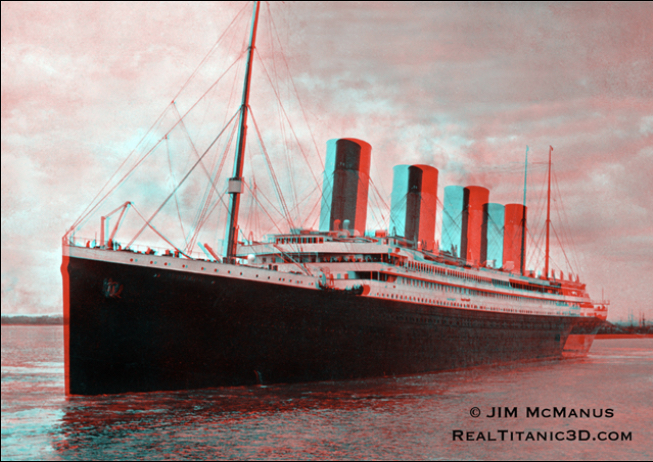
\includegraphics[width=0.5\linewidth]{figures/stereo/titanic.jpg}}
\sublabel{b}{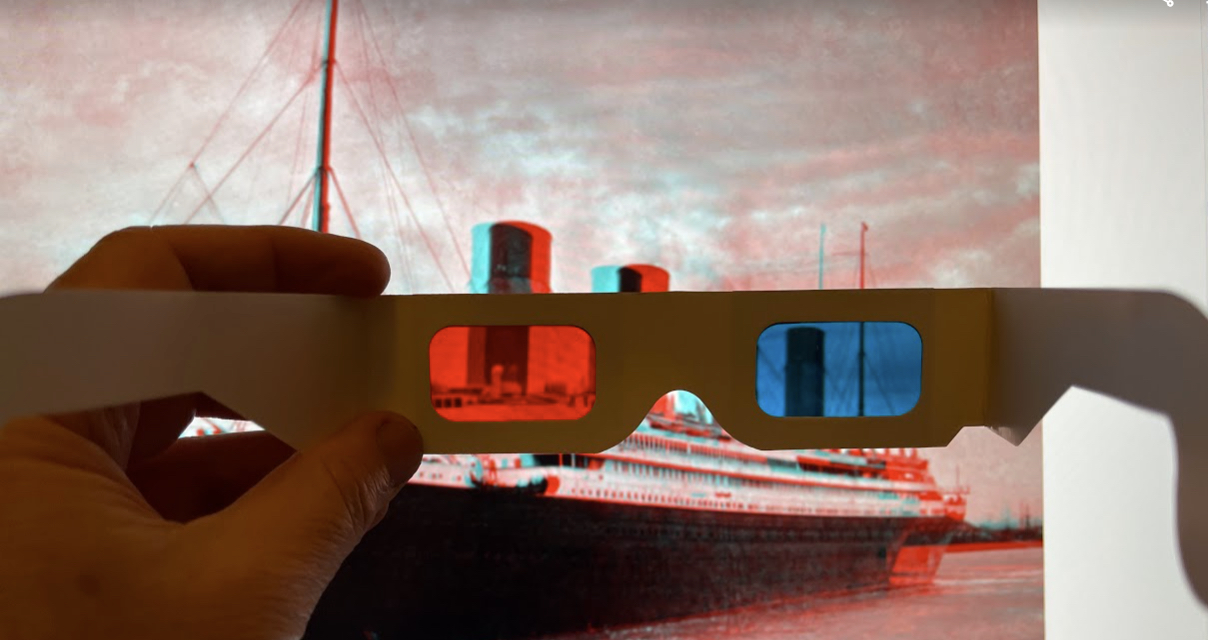
\includegraphics[width=0.5\linewidth]{figures/stereo/stereoglasses.jpg}}}
\caption{(a) Stereo anaglyph of the ocean liner, the Titanic \cite{McManus2022}.  The red image shows the right eye's view, and cyan the left eye's view.  When viewed through stereo red/cyan stereo glasses, as in (b), the cyan variations appear in the left eye image and the red variations appear to the right eye, creating a the perception of 3D.}
\label{fig:titanic}
\end{figure}

Figure~\ref{fig:titanic}~(a) shows a stereo anaglyph of the ill-fated ocean liner, the Titanic, from \cite{McManus2022}.  This was taken with two cameras, one displaced laterally from the other.  The right camera's image appears in red in this image, and the left camera image is in cyan.  If you view this image with a red filter covering the left eye, and a cyan filter covering the right, (b), then the right eye will see only the right camera's image, analogously for the left eye, allowing the ship to pop-out into a 3D stereo image.  Note that the relative displacement between each camera's image of the smokestacks changes as a function of their depth, which allows us to form a 3D interpretation of the ship, when viewing the image with the glasses of Figure~\ref{fig:titanic}~(b).


 In this chapter, we study how to compute depth from a pair of spatially offset camera images, such as those of Fig.~\ref{fig:titanic}.  There are two parts to the depth computation, usually handled separately:  (1) analyzing the geometry of the camera projections, which allows for triangulating depth once image offsets are known, and (2) calculating the offset between matching parts of the objects depicted in each image.  Different techniques are used in each part.  We first address the geometry, asking where points matching those in a first image can lie in the second image. A manipulation, called image rectification, is often used to place the locus of potential matches along a pixel row.  Then, assuming a rectified image pair, we will address the second part of the depth computation, computing the offsets between matching image points.

\section{Stereo Geometry}

\section{Epipolar lines}
\label{sect:epipolar}
\begin{figure}
\centerline{
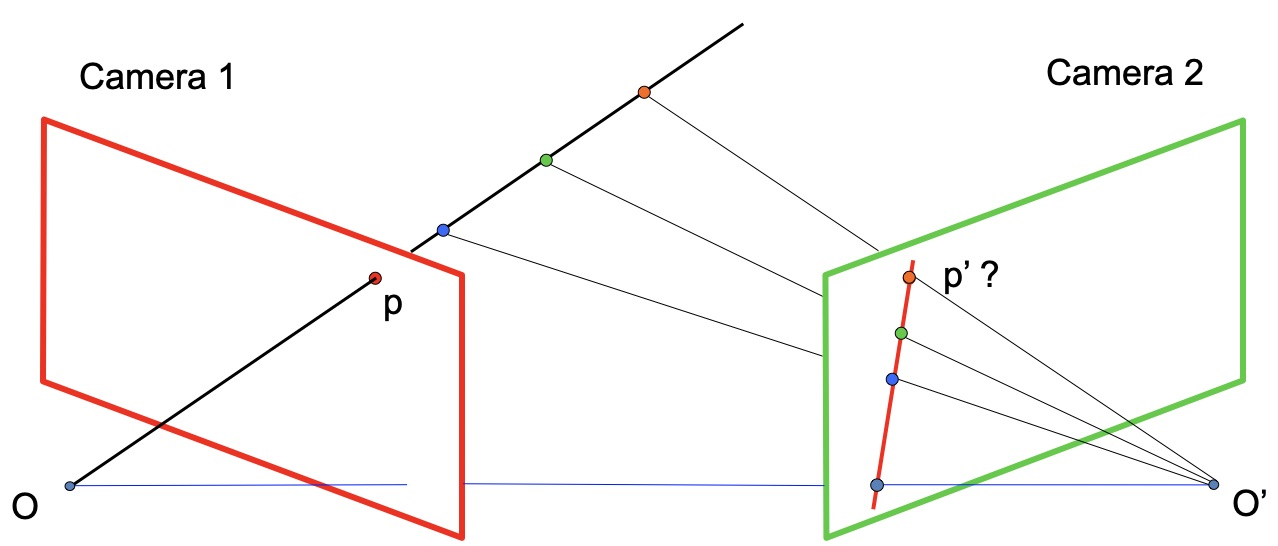
\includegraphics[width=0.8\linewidth]{figures/stereo/epipolar.jpg}
}
\caption{Epipolar lines}
\label{fig:epipolar}
\end{figure}

Knowing where to look for the match for a given feature point in another image can greatly reduce the computational complexity and increase the reliability of the task.  Figure~\ref{fig:epipolar} shows the geometry of the matching task.  A given feature at location p in camera 1 can occur anywhere in depth along the line connecting O (the optical center of camera 1) and the location of the feature point in the virtual sensor point, p.  When each of those possible 3D points is viewed from camera 2, each point will appear on a line in the sensor plane of camera 2, where the plane defined by O, O', and p  intersects the virtual sensor plane of camera 2. This line of candidate stereo matches 
 is called an epipolar line.   To find the stereo match for the point p, we only need to look along the  epipolar line in the image formed by camera 2, \cite{Hartley2004}.

\subsection{Image rectification}
Another application of the homography transformations described in Chapt. YY is a stereo pre-processing step called {\bf image rectification}.  As described above, one only needs to search along epipolar lines to find matching points in the second image.  If the sensor planes of each camera are co-planar, and if the pixel rows are co-linear across the two cameras, then the epipolar lines will be along image scanlines, simplifying the stereo search.  Using the homography transformations, we can warp observed stereo camera images taken under general conditions to synthesize the images that would have been recorded had the cameras been aligned to yield epipolar lines along scan rows.

Many configurations of the two cameras satisfy the desired image rectification constraints \cite{Zhang2003}: (a) that epipolar lines are along image scanlines, and (b) matching points are within the same rows in each camera image.  One procedure that will satisfy those constraints is as follows \cite{wikiRectification}:  

First, use Eq.~(\ref{eq:homographyRotation}) to rotate each camera to be parallel with each other and with optical axes perpendicular to the line joining the two camera centers.  Second, rotate each of the cameras about its optical axis to align the rows of each camera with those of the other.  Third, uniformly scale one camera's image to be the same size as to the other, if necessary.  The resulting image pair will satisfy the two requirements above for image rectification.

Others algorithms are optimized to minimize image distortions \cite{Zhang2003} and may give better performance for stereo algorithms.  We assume camera calibrations are known, but other rectification algorithm can require only weaker conditions, such as knowing the fundamental matrix \cite{Hartley2004,Pollefeys99}. Many software packages provide image rectification code, \cite{github2022}.




\section{Stereo triangulation}

For the rest of this chapter, we will assume our stereo camera images are rectified, and we only need to look along a given scan line to find the matching position of any given point of one stereo image in the second stereo image.

\begin{figure}
\centerline{
\sublabel{a}{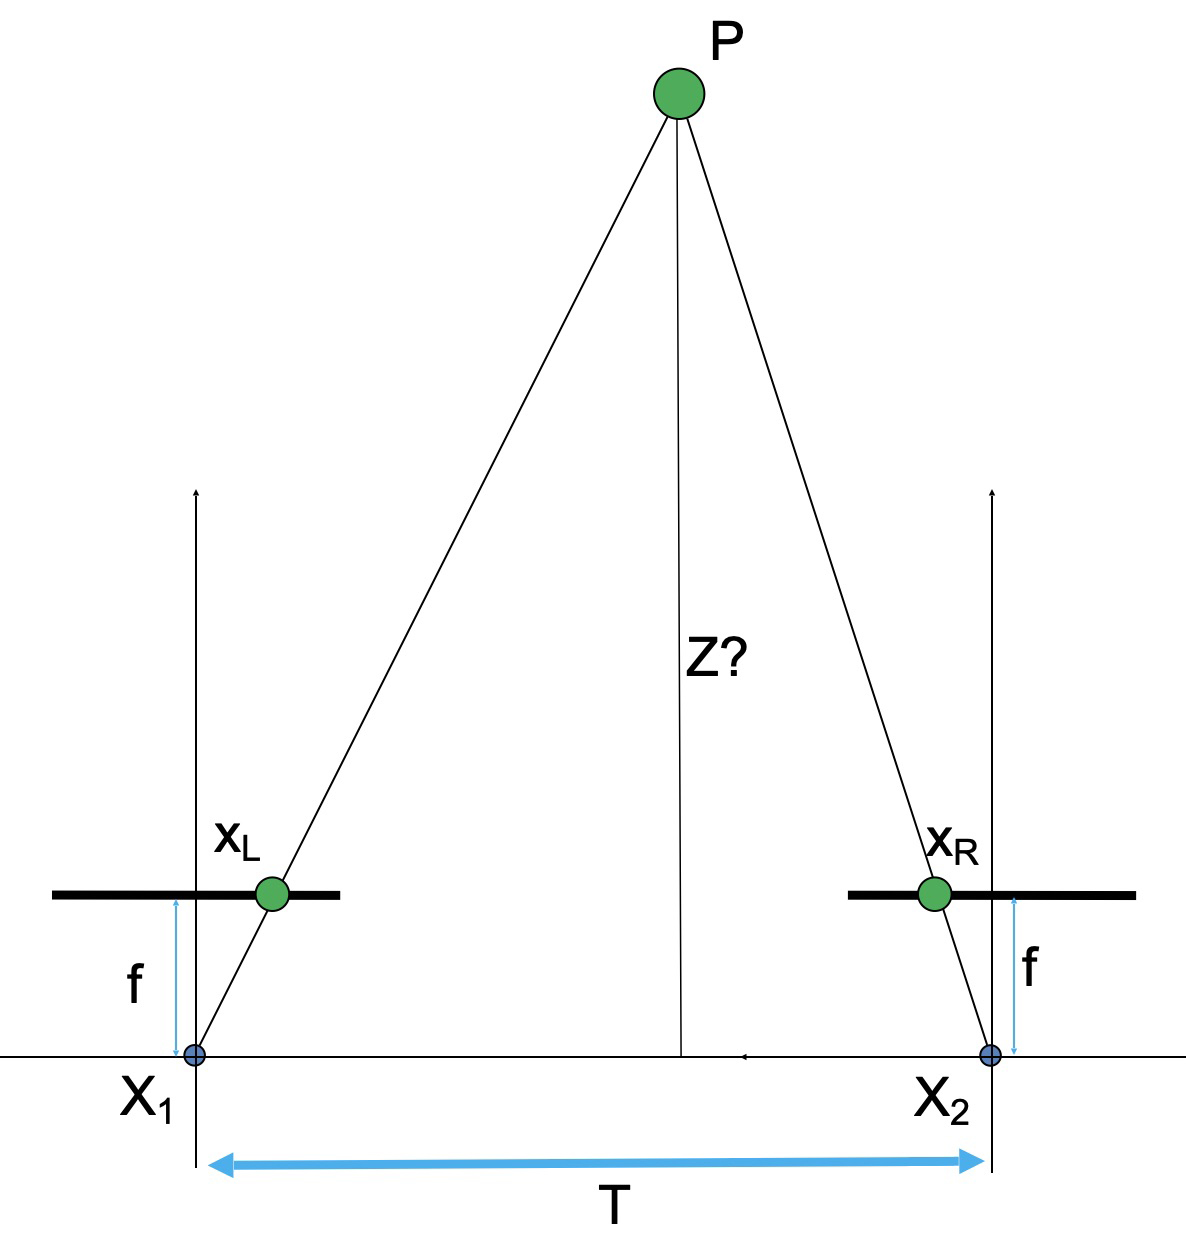
\includegraphics[width=0.4\linewidth]{figures/stereo/stereo.jpg}}}
\centerline{
\sublabel{b}{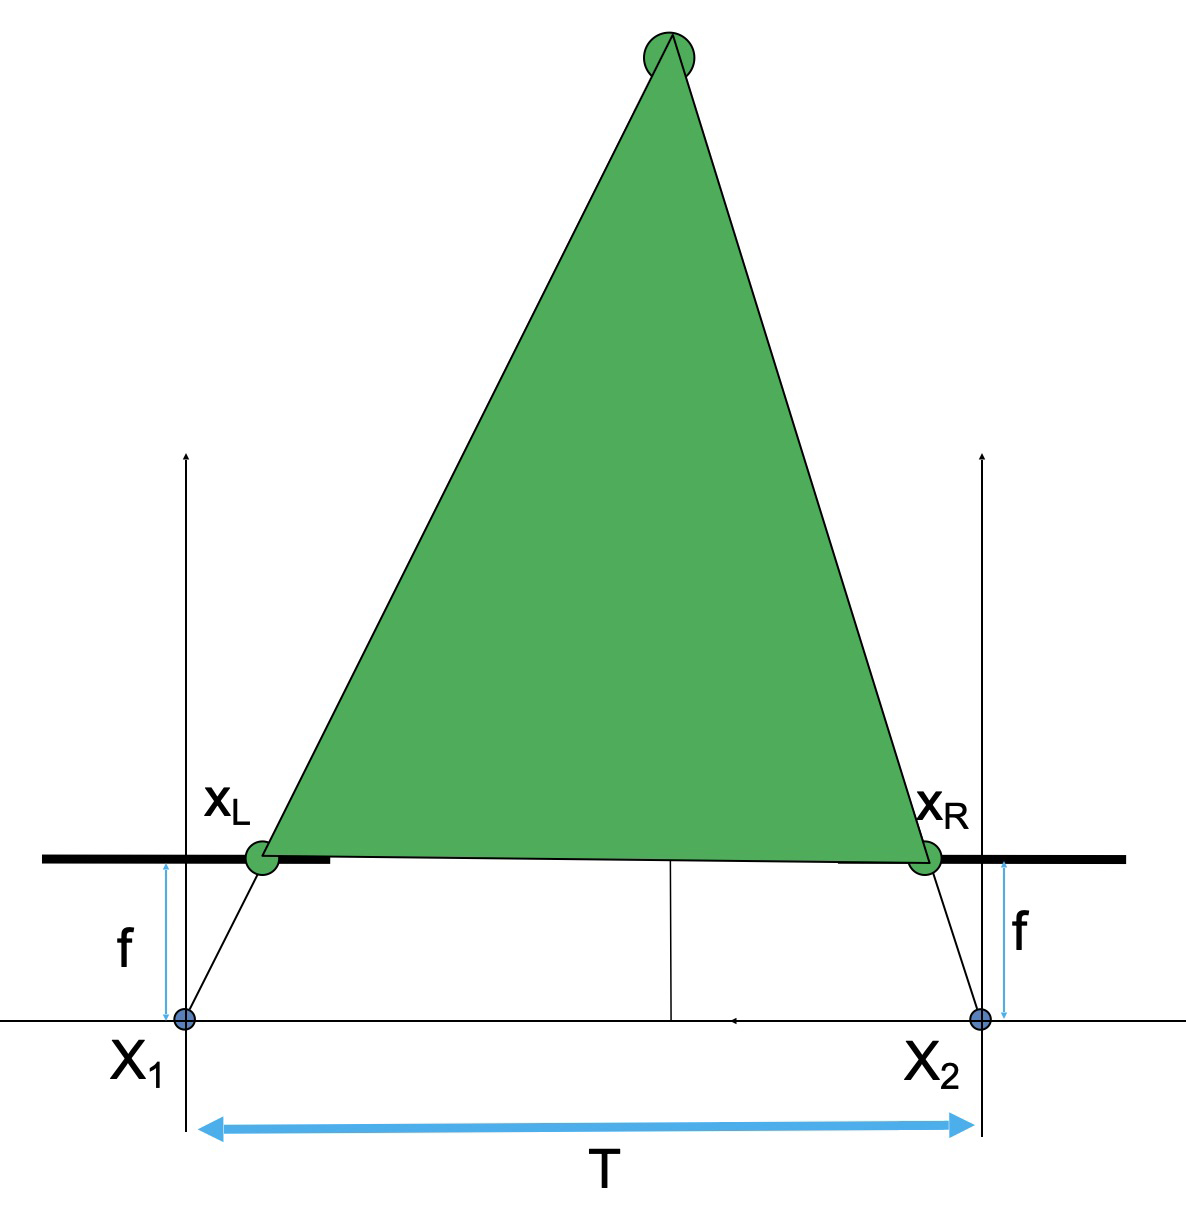
\includegraphics[width=0.4\linewidth]{figures/stereo/stereoGreen.jpg}}
\sublabel{c}{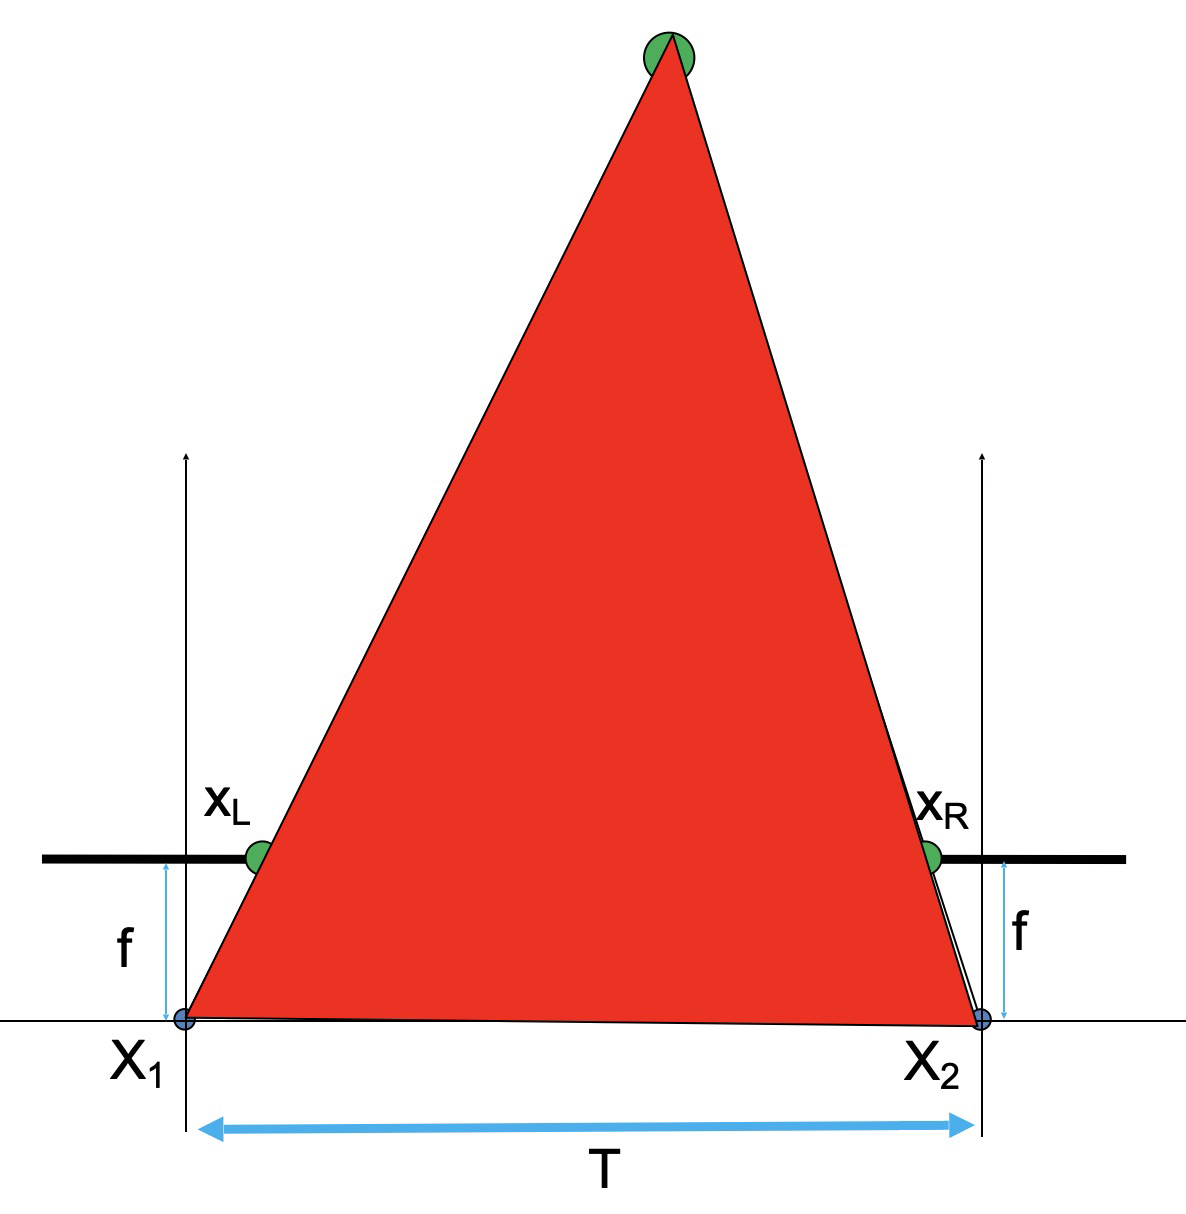
\includegraphics[width=0.4\linewidth]{figures/stereo/stereoRed.jpg}}
}
\caption{Depth triangulation from stereo. (a) Two cameras, of identical focal length, f, and separated by an offset, T, image the point P onto $X_1$ and $X_2$ at camera.  The similarity of the two triangles in (b) and (c) leads to Eq.~(\ref{eq:depthFromDisparity}) for the depth, Z, of the point P.}
\label{fig:stereo}
\end{figure}

The task of stereo is to triangulate the depth of points in the world by comparing the images from two spatially offset cameras.  (If more than two cameras are used, the task is referred to as multi-view stereo).  To triangulate depth, we need to describe how image positions in the stereo pair relate to depth in the 3d world. 


The geometry shown in Fig.~\ref{fig:stereo} reveals the essence of depth estimation from a pair of rectified cameras.   The two cameras are centered  at horizontal positions $X_1$ and $X_2$, respectively, and are identical and are oriented with their optical axes parallel with each other.  We consider the depth estimate within a single image row.  To distinguish 2d image coordinates from 3d world coordinates, for this chapter, we will denote 2-d image coordinates by lower-case letters, and 3-d world coordinates by upper-case letters. The green circle at point P, for which we want to estimate the depth, Z, appears in the left camera at position $X_L$ and in the right camera at position $X_R$.  

A simple way to triangulate the depth, Z, of a point visible in both images is through similar triangles.  The two triangles shown in  Fig.~\ref{fig:stereo}~(b) and (c) are similar, and so the ratios of their height to base must be the same.  Thus we have:
\begin{equation}
    \frac{T+X_R-X_L}{Z-f} = \frac{T}{Z}
\end{equation}
Solving for Z gives:
\begin{equation}
    Z = f \frac{T}{X_L-X_R}
    \label{eq:depthFromDisparity}
\end{equation}
The difference in horizontal position of any given world point, P, as seen in the left and right camera images, $X_L - X_R$, is called the {\bf disparity}, and is {\em inversely proportional to the depth} Z of the point P for this configuration of the two cameras--parallel orientation.  The task of inferring depth of any point in either image of a stereo pair thus reduces to measuring the disparity everywhere.

In closing, we note that disparity of the smokestacks in Fig.~\ref{fig:titanic}~(a) increases with depth, rather than decreasing as described by Eq.~(\ref{eq:depthFromDisparity}).  That is because the cameras that took the stereo pair were not in the same orientation, related only by a translation.  After rectification, the stereo image pair of Fig.~\ref{fig:titanic}~(a) would obey the depth-disparity relation of Eq.~(\ref{eq:depthFromDisparity}).



\subsection{Stereo Matching}
Now we know where to look for stereo matches (along corresponding scanlines in rectified image pairs), and we know how the stereo disparity relates to depth (inversely proportional).  We just need to locate the positions of matching points in the stereo pair to estimate their depth.

First, let's examine the task visually.   Figure~\ref{fig:stereomatch} shows two images of an office, take approximately one meter apart.  The locations of several objects in the left image, (a), are shown in the right image, (b), revealing some of the disparities that we seek to measure automatically.  As the reader can appreciate by comparing the stereo images by eye, one can compute the disparity by first localizing a feature point in one image and then finding the corresponding point in the other image, based on the visual similarity of the local image region.  To do this automatically is the crux of the stereo problem.


\begin{figure}
\centerline{
\sublabel{a}{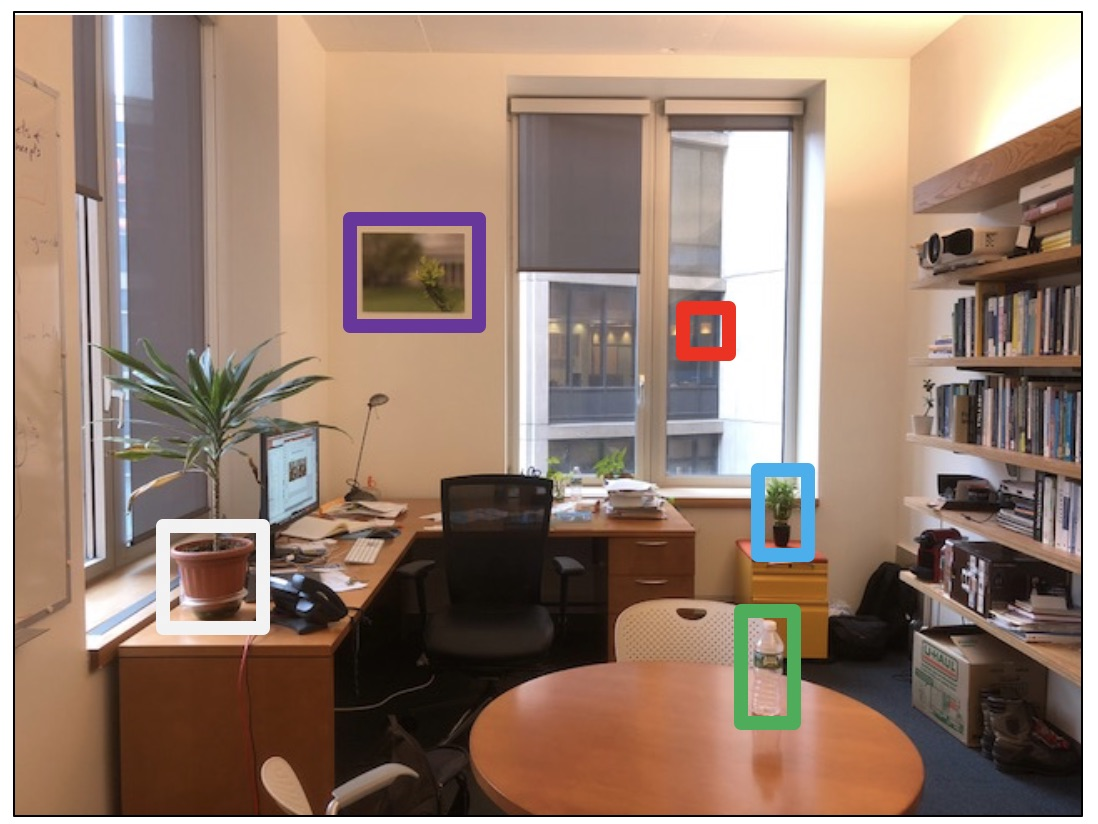
\includegraphics[width=0.5\linewidth]{figures/stereo/officeLeft.jpg}}
\sublabel{b}{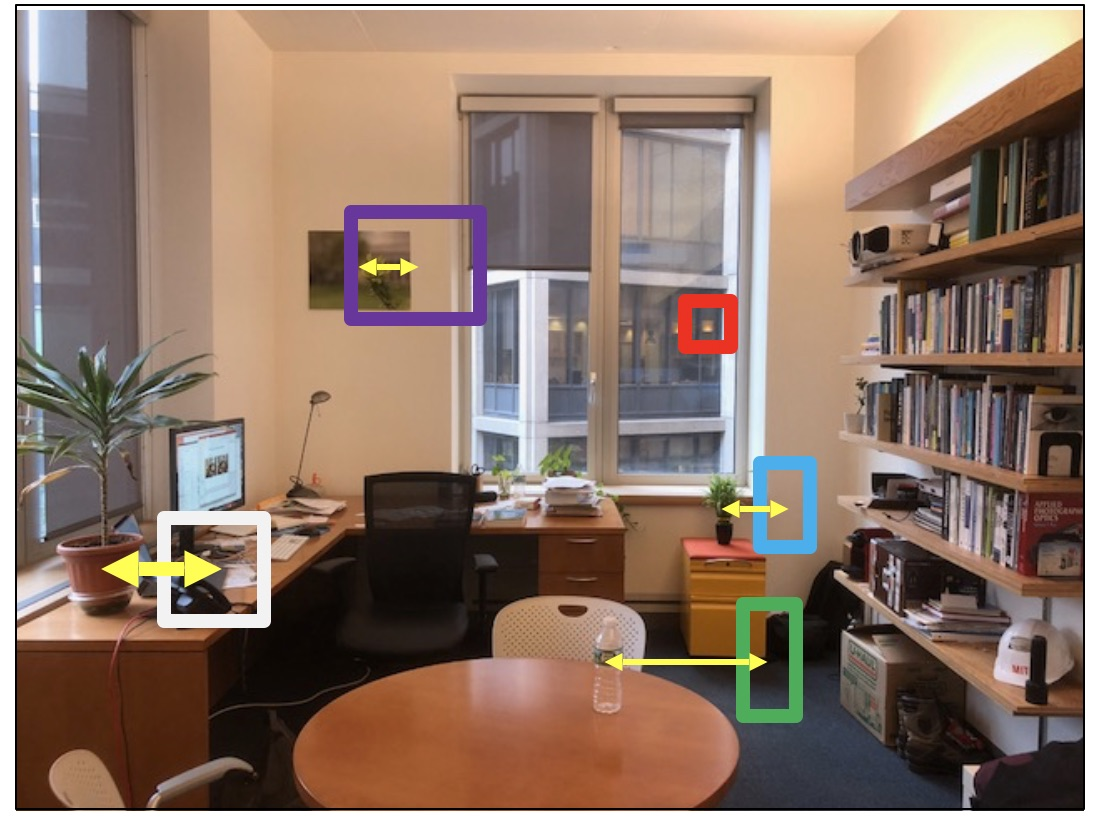
\includegraphics[width=0.5\linewidth]{figures/stereo/officeRight.jpg}}
}
\caption{Two cameras, displaced from each other laterally, photograph the same scene, resulting in images (a) and (b).  Colored rectangles show some identifiable features in image (s), and where those features appear in image (b).  Arrows show the corresponding displacements, which reveal depth through Eq.~(\ref{eq:depthFromDisparity})}.
\label{fig:stereomatch}
\end{figure}


A naive algorithm for finding the disparity of any pixel in the left image is to search for a pixel of the same intensity  in the corresponding row of the right image.  Figure~\ref{fig:stereolamp}, from \cite{Hosni2013}, shows why that naive algorithm won't work, and why this problem is hard.  (a) shows the intensities of one row of the right eye image of a stereo pair. The squared difference of the intensity differences from offset versions of the same row in the rectified left eye image of the stereo pair is shown in (b), for a range of disparity offsets, plotted vertically, in a configuration known as the disparity space image \cite{Scharstein2002}.  The disparity corresponding to the minimum squared error matches are plotted in red.  Note the disparities of the best pixel intensity matches show much more disparity variations than would result from the smooth surfaces depicted in the image; the local intensity matches don't reliably indicate the disparity.  Many effects lead to that unreliability, including: lack of texture in the image, leading to noisy matches among the many nearly identical pixels; image intensity noise; specularities in the image which change location from one camera view to another; and scene points appearing in one image but not another due to occlusion. (d) shows an effective approach to remove the matching noise:  blurring the disparity space image using an edge-preserving filter \cite{Hosni2013}.  The best-matching disparities are plotted in red, and compare well with (f) the ground truth disparities, as labeled in the dataset \cite{Scharstein2002}.

\begin{figure}
\centerline{
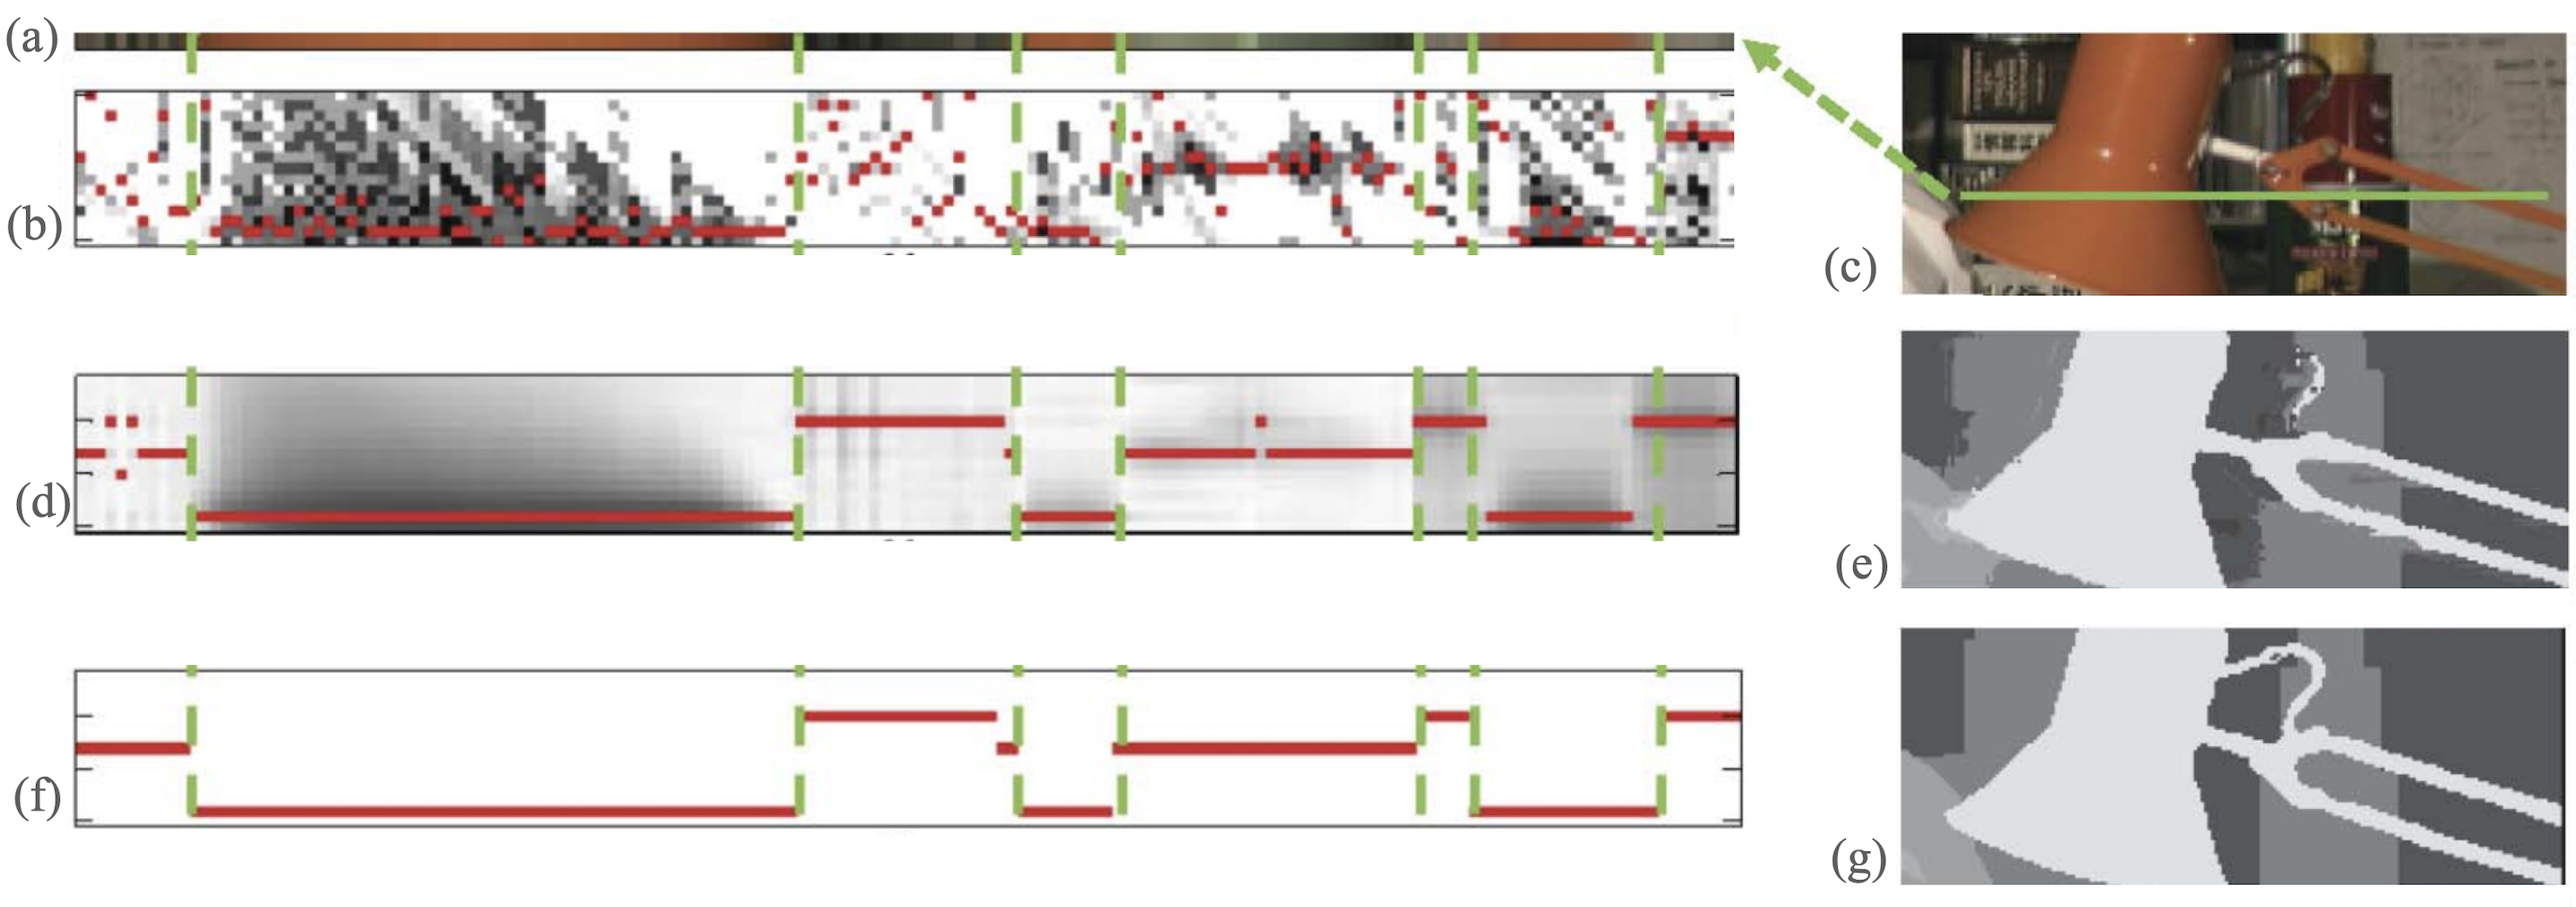
\includegraphics[width=0.9\linewidth]{figures/stereo/stereolamp.jpg}}
\caption{Intensity-based stereo matching issues. (a) Intensities of scanline of one image, (c), of stereo pair. (b) Intensity matching error for different disparities, plotted vertically, as a function of horizontal position.  Disparities of best intensity match shown in red. (d) Smoothing the disparity cost volume yields better matches, shown in red. (e) Resulting depth image.  (f) Ground truth disparities and (g) depth image, from dataset by  \cite{Scharstein2002}. Figure reprinted and modified from \cite{Hosni2013}, permissions to be obtained}
\label{fig:stereolamp}
\end{figure}

The task of finding disparity at each point is often broken into two parts:  (a) finding features, and matching the features across images, and (b) interpolating between, or adjusting, the feature matches to obtain a reliable disparity estimate everywhere.
These two steps are often called matching and filtering, because the interpolation can be performed using filtering methods.



\section{Finding image features}
Good image features are positions in the image that are easy to localize, given only the image intensities. The Harris corner \cite{Harris88} algorithm identifies image points that are easy to localize by evaluating how the sum of squared intensity differences over an image patch change under a small translation of the image. If the squared intensity changes quickly with patch translation in every direction, then the region contains a good image feature. 

Let the image be $x[n,m]$, and let the small translation be $\delta n$ in $n$ and $\delta m$ in $m$.  Then the squared intensity difference, $E(\delta n, \delta m)$ induced by that small translation, summed over a small patch, will be
\begin{equation}
    E(\delta n, \delta m) = \Sigma_{(n, m) \in P}
    (x[n,m] - x[n + \delta n, m + \delta m])^2
    \label{eq:harris}
\end{equation}

We expand $x[n + \delta n, m + \delta m]$ about $x[n, m]$ in a Taylor series:
\begin{equation}
    x[n + \delta n, m + \delta m] \approx
    x[n, m] + \frac{\partial x}{\partial n} \delta n
    + \frac{\partial x}{\partial m} \delta m
\end{equation}
Substituting the above into Eq.~\ref{eq:harris} and writing the result in matrix form yields
\begin{equation}
       E(\delta n, \delta m) \approx
       \left( \begin{array}{c c}
       \delta n & \delta m
       \end{array}
       \right)
       \mathbf{M} 
       \left( \begin{array}{c}
       \delta n \\
       \delta m
       \end{array}
       \right) 
\end{equation}
where
\begin{equation}
\mathbf{M} = \Sigma_{(n, m) \in P}
\left( \begin{array}{c c}
(\frac{\partial x}{\partial n})^2 & 
\frac{\partial x}{\partial n} 
\frac{\partial x}{\partial m} \\
\frac{\partial x}{\partial n} 
\frac{\partial x}{\partial m} 
& (\frac{\partial x}{\partial m})^2
\end{array} \right)
\end{equation}

The smallest eigenvalue, $\lambda_{\mbox{min}}$ of the matrix, $\mathbf{M}$, indicates the smallest possible change of image intensities under translation of the patch in any direction.  Thus, to detect good corners, one can identify all points for which $\lambda_{\mbox{min}} > \lambda_c$, for some threshold $\lambda_c$.
The Harris corner detector has been widely used for identifying features to match across images, although they were later supplanted by SIFT features \cite{Lowe04}, based on maxima over scale of Laplacian filter outputs.  Figure~\ref{fig:stereopoints}~(a) and (b) show the result of the Harris feature detector to the images of Fig.~\ref{fig:stereomatch}.


\begin{figure}
\centerline{
\sublabel{a}{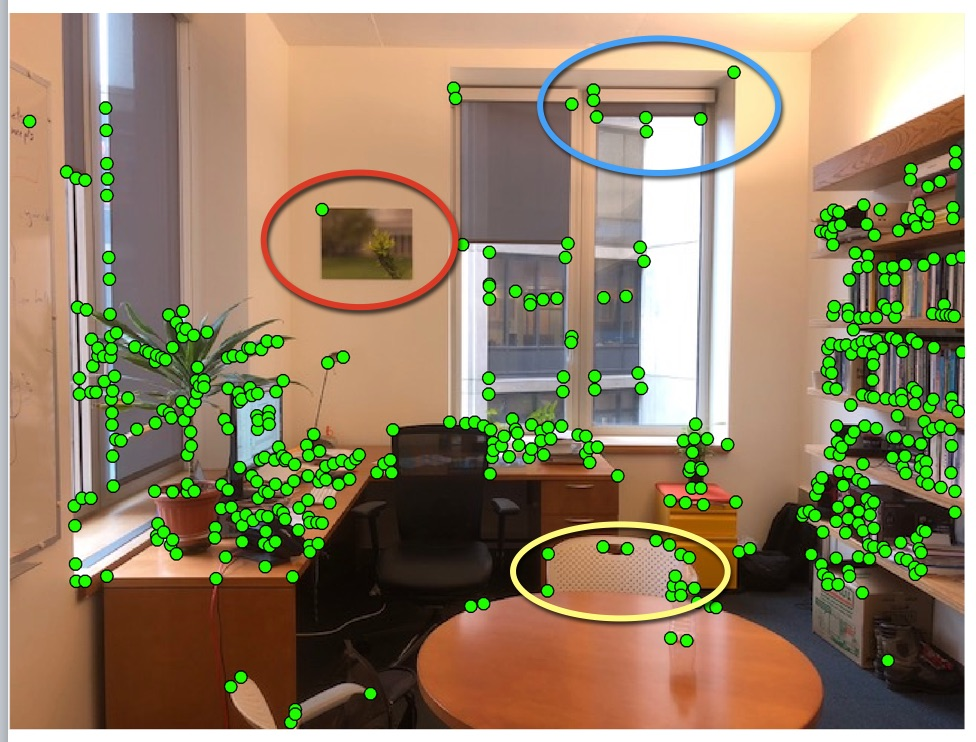
\includegraphics[width=0.4\linewidth]{figures/stereo/pointsLeft.jpg}}
\sublabel{b}{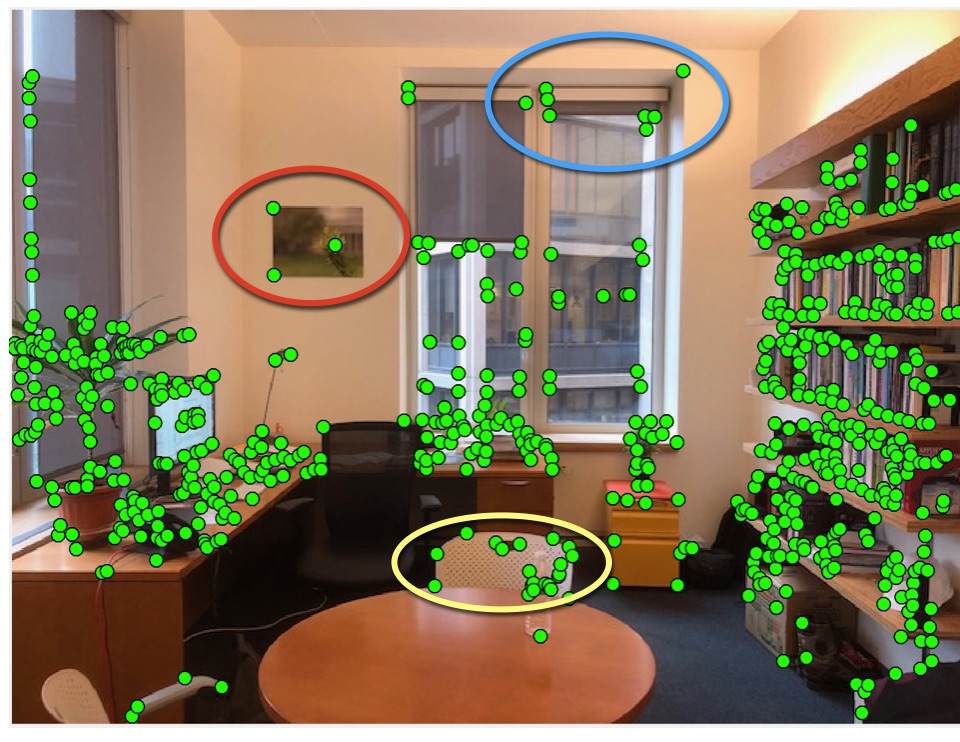
\includegraphics[width=0.4\linewidth]{figures/stereo/pointsRight.jpg}}
\sublabel{c}{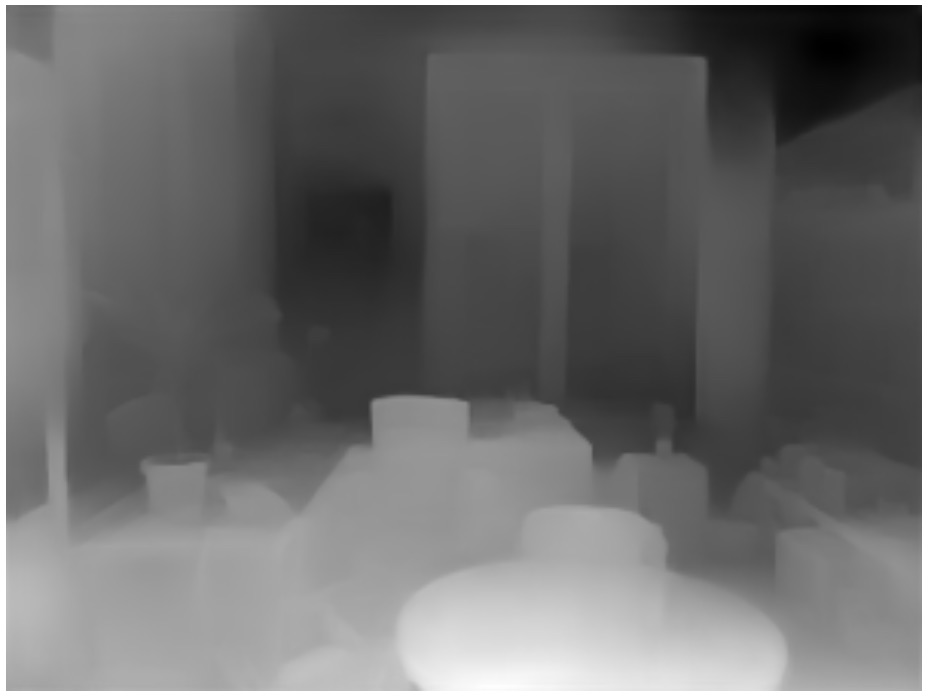
\includegraphics[width=0.4\linewidth]{figures/stereo/officeDepth.jpg}}
}
\caption{The feature-based stereo approach, illustrated for the stereo pair of Fig.~\ref{fig:stereomatch}.  Feature points are found, independently, in each of the stereo pair images (a) and (b).  Detected Harris feature points \cite{Harris1988} are shown as green dots. It is especially visible within the marked ellipses that not the same set of feature points is marked in each image.  (c) shows a depth image resulting from a matched and interpolated set of feature points.}
\label{fig:stereopoints}
\end{figure}

Figure~\ref{fig:stereopoints}~(a) and (b) reveal the challenges of the feature matching task:  (1) not every feature is marked across both images, and (2) we need to decide which pairs of image features go together.  

\section{Local Image Descriptors}

Matching corresponding image features requires a local description of the image region to allow matching like regions across two images.  SIFT features  \cite{Lowe04} use histograms of oriented filter responses to create an image descriptor which is sensitive to local image structure, but which is insensitive to minor changes in lighting or location which may occur across the two images of a stereo pair.


\begin{figure}
\centerline{
\sublabel{a}{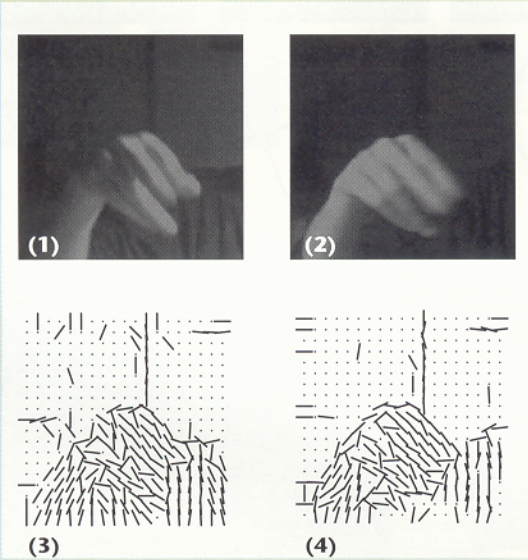
\includegraphics[width=0.4\linewidth]{figures/stereo/hands.jpg}}
\sublabel{b}{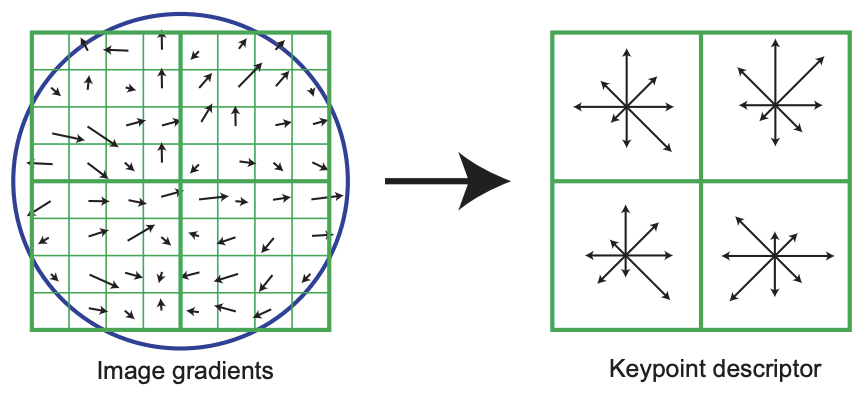
\includegraphics[width=0.5\linewidth]{figures/stereo/SIFT.jpg}}
}
\caption{Orientation-based image descriptors.  (a) Top row:  two images of a hand under different lighting conditions look quite different in a pixel intensity representation, but, Bottom row, look quite similar in a local orientation, depicted by line segment directions.  Reprinted from \cite{Freeman98c}.  SIFT image descriptors \cite{Lowe04} exploit that observation.  Taking (b) histograms of local orientation over local spatial regions further allow for image descriptors to be robust to small image translations \cite{Freeman98c,Lowe04}.  }
\label{fig:SIFT}
\end{figure}

\section{Interpolation between feature matches}
Methods to interpolate depth between the depths of matched points include probabilistic methods such as belief propagation, discussed in chapter~\ref{chapt:InferenceInGraphicalModels}.  Under assumptions about the local spatial relationships between depth values, optimal shapes can be inferred provided the spatial structure over which inference is performed is a chain or a tree.  \cite{Hirschmuller2007} uses a related inference algorithm, dynamic programming, which has the same constraints on spatial structure for exact inference.  Hirschmuller's algorithm, called Semi-Global Matching (SGM), applies the 1D processing over many different orientations to approximate a global solution to the stereo shape inference problem.

\section{Neural Network Stereo Algorithms}
As is the case for most other vision tasks, neural network approaches now dominate stereo methods.  The two stages of a stereo algorithm, matching and filtering, can be implemented separately by neural networks (eg, \cite{Zbontar2015}), or together in a single, end-to-end optimization (\cite{Zhang2019GANet,Chang2018,Mayer2016,Kendall2017}.

A common approach, depicted in block diagram form in Fig.~\ref{fig:stereoblock}, is the following:
\begin{itemize}
    \item Rectify the stereo pair so that scanlines in each image depict the same points in the world.
    \item Extract features from each image, using a pair of networks with shared weights.
    \item Form a 3d cost volume (see Fig.~\ref{fig:stereoLamp}) indicating the local visual evidence of a match between the two images for each possible pixel position and each possible stereo disparity.  (This 3D cost volume can be referenced to the H and V positions of one of the input images.)
    \item Train and apply a 3D CNN to aggregate (process) the costs over the 3D cost volume in order to estimate a single, best disparity estimate for each pixel position.  This performs the function of the regularization step of non-neural-network approaches, such as SGM \cite{Hirschmuller2007}, but the performance is better for the neural network approaches.
\end{itemize}


\begin{figure}
\centerline{
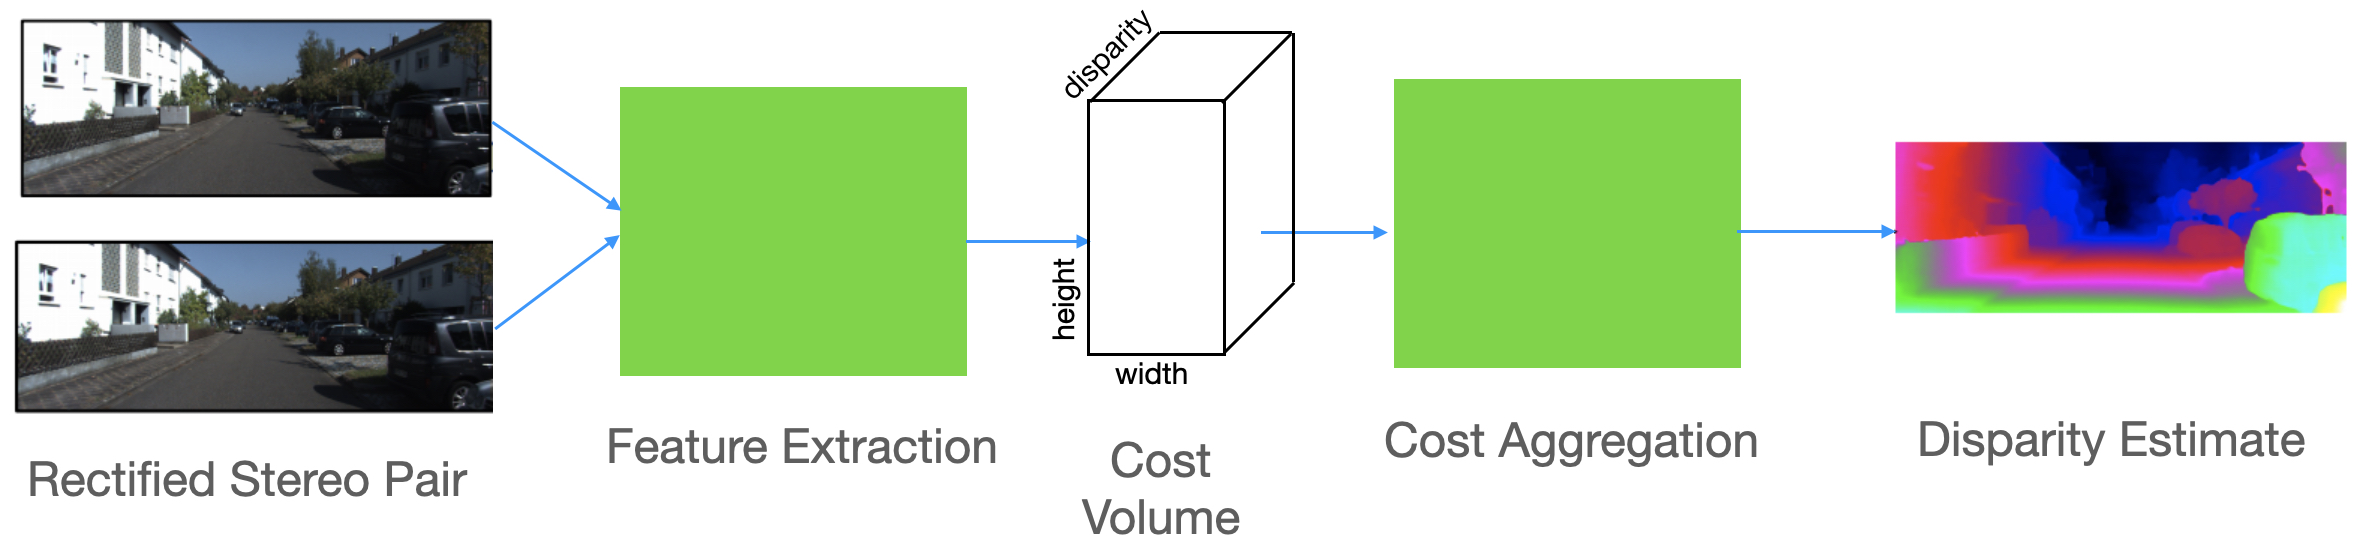
\includegraphics[width=0.8\linewidth]{figures/stereo/stereocnn.jpg}
}
\caption{Block diagram of CNN stereo processing, abstracted from the block diagrams of \cite{Chang2018,Zhang2019GANet,Kendall2017}.}
\label{fig:stereoblock}
\end{figure}

The performance of methods following the block diagram of Fig.~\ref{fig:stereoblock} surpassed that of previous methods.  More recent work has addressed the problem of poor generalization to out-of-training-domain test examples \cite{zhang2019domaininvariant}.  Training and computing the 3d neural network to process the cost volume can be expensive in time and memory and recent work has obtained both speed and performance improvement through developing an iterative algorithm to avoid the 3D filtering \cite{Lipson2021}.


\section{Comparing the performance of stereo algorithms}
The "Middlebury Stereo web page" \cite{Scharstein2002} provides a comprehensive comparison of many stereo algorithms, compared on a common dataset, with pointers to algorithm descriptions and code.  One can use the web page to evaluate the improvement of stereo reconstruction algorithms over time.  The advancement of the field over time is very impressive.


